\documentclass[a4paper, 11pt]{article}
\usepackage[a4paper,left=2cm,right=2cm,top=1.8cm,bottom=2.8cm]{geometry}
\usepackage[english]{babel}
\usepackage{pictex,amsmath,amsfonts,amssymb,amsthm,verbatim}
\usepackage{fullpage}
\usepackage{fullpage}
\usepackage{fancyhdr}
\usepackage{algorithm,algorithmic}
\usepackage{multirow}
\usepackage{gensymb}
\usepackage{mathrsfs}
\usepackage{hyperref}

\setlength{\voffset}{-0.25in}
\setlength{\headsep}{+0.5in}
\setlength{\parskip}{1em}
\setlength{\parindent}{0em}

\def\vu{\mathbf{u}}
\def\vv{\mathbf{v}}
\def\vb{\mathbf{b}}
\def\vw{\mathbf{w}}
\def\vs{\mathbf{s}}

%Bibliography
%\usepackage[backend = biber, style = authoryear]{biblatex}
%\addbibresource{HelloWorld.bib}
\usepackage{etoolbox}
\patchcmd{\thebibliography}{\section*{\refname}}{}{}{}

%Graphics packages:
\usepackage{graphicx, graphics}
\usepackage{tabularx, caption}
\usepackage{multirow, multicol}
\usepackage{setspace, tikz}
\usepackage{xcolor}
\usepackage{titlesec}
\usepackage{mdframed}
\usepackage{fancyhdr}
\usepackage{lastpage}
\usepackage[utf8]{inputenc}

\newmdenv[linecolor=blue,skipabove=\topsep,skipbelow=\topsep,leftmargin=5pt,rightmargin=-5pt,innerleftmargin=5pt,innerrightmargin=5pt]{mybox}

\newcommand{\quotes}[1]{``#1''}


\usepackage{minted}
\newminted{C}{frame = lines, framerule = 2pt}


%fancyhdr:
\setlength{\headheight}{40pt}
\pagestyle{fancy}
\fancyhead{} % clear all header fields
\fancyhead[L]{
 \begin{tabular}{rl}
    \begin{picture}(25, 15)(0, 0)
    \put(0, -8){
\includegraphics[width=8mm, height=8mm]{hcmut.png}}
   \end{picture}&
	\begin{tabular}{l}
		\textbf{\bf \ttfamily University of Technology, VNU-HCM}\\
		\textbf{\bf \ttfamily Faculty of Computer Science \& Engineering}
	\end{tabular} 	
 \end{tabular}
}

\fancyhead[R]{
    \begin{tabular}{l}
        \tiny \bf \\
        \tiny \bf
    \end{tabular}
}

\fancyfoot{} %clear all footer fields
\fancyfoot[L]{\scriptsize \ttfamily CC01 - Operating System (Spring 2019)}
\fancyfoot[R]{\scriptsize \ttfamily Page {\thepage}/ \pageref{LastPage}}
\renewcommand{\headrulewidth}{0.3pt}
\renewcommand{\footrulewidth}{0.3pt}

\begin{document}
    \begin{titlepage}
        \begin{center}
            HO CHI MINH CITY UNIVERSITY OF TECHNOLOGY, VNU HCM \\
            FACULTY OF COMPUTER SCIENCE AND ENGINEERING
        \end{center}

        \vspace{1cm}

        \begin{figure}[h!]
            \begin{center}
                
\includegraphics[width=3cm]{hcmut.png}
            \end{center}
        \end{figure}

        \vspace{1cm}

        \begin{center}
            \begin{tabular}{c}
                \multicolumn{1}{l}{\textbf{\LARGE OPERATING SYSTEM}} \\
                ~~\\
                \hline
                \\
                \multicolumn{1}{l}{\LARGE Assignment \#1: System Call} \\
                \\
                \hline
                \\
                \hspace{5cm} Pham Minh Tuan - MSSV: 1752595
            \end{tabular}
        \end{center}
    \end{titlepage}

%Newpage:
\newpage

\renewcommand*\contentsname{Contents:}
\tableofcontents

\newpage
\section{Introduction:}
\subsection{System Call:}

\par{In computer, a system call is controlled entry point into a kernel, allowing a process to request that the kernel perform some action on the process's behalf. The kernel will make a range of services accessible to programs via system call as application programming interface (API)}.

\begin{itemize}
    \item A system call changes the processor state from \textbf{user mode} to \textbf{kernel mode}, so that CPU can access protected kernel memory.
    \item The set of system calls is fixed. Each system call is identified by a unique number.
    \item Each system call may have a set of arguments that specify information to be transferred from \textbf{user space} to \textbf{kernel space} and vice versa.
\end{itemize}

\bigbreak

\par{This assignment requires to create a system call named \textbf{procmem} to show users about the memory layout of specific process. I will go briefly into each step about preparing my virtual machine, compiling kernel and embedded a new system call.}

\newpage
\section{Preparing Virtual Machine}
\subsection{VM Ware:}

\par{To prepare the new virtual machine for doing assignment 1, I choose to use the one given by lecturer in the link: \url{https://drive.google.com/file/d/15A2N4H_vx-wMkIhP2kG0fkfHE3K5MqwJ/view?usp=sharing}.}

\par{However I came with the biggest problem when trying to run update commmand due to specific errors related to current packages:}

\bigbreak
\includegraphics[scale = 0.7]{error_given_vm.png}
\bigbreak

\par{It say that the I need to use the CDROM available with apt. However I came to the solution to solve this problem by upgrade it into the latest version by 18.04.2 LTS instead of the current 16.04 LTS by running upgrade command:}

\begin{minted}{bash}
    $ sudo do-release-update
\end{minted}

\par{And it also require the sudo priviledge to execute the command. After the upgrade process finished, I rebooted the virtual machine and everything seems fine since all packages is now updated automatically and up-to-date thourgh upgrading.} 

\par{I followed the instructions in the assignment to install toolchains (gcc, make, etc) and the kernel-package}.

\textbf{QUESTION:} Why do we need to install kernel package ? \\
\textbf{Ans:} We need to install kernel-package to easily manage all versions of kernel in virtual machine and install it rightfully, also it allow you to keep multiple of linux images without fuss.

\bigbreak
\subsection{Create and Download Kernel source:}

\par{The kernel compilation folder is created in \textit{home} directory. For the source of downloading kernel: \url{ http://www.kernel.org}, I choose to download the version of kernel exactly same as the instruction of Assignment}

\par{Moreover, the version of kernel downloaded is older than the current one running in my virtual machine since I already upgrade it to the latest as well as the kernel, so I will explain specificly about that problem after install the new kernel into the virtual machine.}

\textbf{QUESTION:} Why do we have to use another kernel source from the server such as \url{http://www.kernel.org},
can we just compile the original kernel (the local kernel on the running OS) directly? \\
\textbf{Ans:} The answer is yes, you can compile directly from your current kernel. However in some situations, you need to use the other kernel instead of the current one:
\begin{itemize}
    \item To enable experimental features that are not part of the default kernel.
    \item To enable support for a new hardware that is not currently supported by the default kernel.
    \item To debug the kernel.
    \item Study purpose.
\end{itemize}

\par{After the downloading is complete, you can unpack zip file. Beside, it is recommend that we can install the \textit{openssl libssl-dev} initially.}

\bigbreak
\subsection{Configuration}

\par{In this step, I just follow every instruction in the Assignment to finish the config for the downloaded kernel and change the name of the kernel following by my student ID.}


\section{Kernel Module:}

\subsection{Data Structure:}

\par{In this assignemnt, I was recommend to use the \texttt{task\_struct} and \texttt{mm\_struct}:}

\begin{itemize}
    \item Each process running under a Linux machine is associated with a struct \texttt{task\_struct}. The source code of \texttt{task\_struct} can be read \href{https://github.com/torvalds/linux/blob/a13f0655503a4a89df67fdc7cac6a7810795d4b3/include/linux/sched.h#L585}{here}.
    \item Inside a \texttt{task\_struct}, there is a struct \texttt{mm\_struct} which stores the description of memory of the process. The source code of \texttt{mm\_struct} can be read \href{https://github.com/torvalds/linux/blob/a13f0655503a4a89df67fdc7cac6a7810795d4b3/include/linux/mm_types.h#L351}{here}.
\end{itemize}

\subsection{Create Procmem Kernel Module:}

\par{Modules are pieces of code that can be loaded and unloaded into the kernel upon demand. They can extend the functionality of the kernel without rebooting the system.}

\par{One requirement of the assignment is to write a module to test \textit{procmem} system call. Below is how I implement it:}
\bigbreak

\begin{minted}[frame = single, framesep = 10pt, breaklines, linenos]{C}
#include <linux/module.h> 
// included for all kernel modules

#include <linux/kernel.h> 
// included for KERN_INFO
#include <linux/init.h>
// included for __init and __exit macros

#include <linux/mm.h>
#include <linux/sched/signal.h>
#include <linux/delay.h>

MODULE_LICENSE("GPL");
MODULE_AUTHOR("TUAN");

static int pid = 1;
static int __init procmem_init(void){
    struct task_struct *task;
    printk(KERN_INFO "Starting kernel module!\n");

    // TODO: find task_struct that is associated with the input process pid
    // Hint: use the for_each_process() function:
    for_each_process(task)
    {
        printk("[%d] | [%s]\n", task->pid, task->comm);
        msleep(10);

        if (task->pid == pid)
        {
            printk("Student ID: 1752595\n");

            //check if mm is NULL or not:
            if (task->mm != NULL)
            {
                printk(KERN_INFO "task->mm not null !\n");

                // TODO: show its memory layout
                printk("Code Segment start = [%lu]; end  = [%lu]\n", task->mm->start_code, task->mm->end_code);
                printk("Data Segment start = [%lu]; end  = [%lu]\n", task->mm->start_data, task->mm->end_data);
                printk("Stack Segment start = [%lu]\n", task->mm->start_stack);

                return 0;
            }

            else if (task->active_mm == NULL)
            {
                printk(KERN_INFO "In the thread, using active_mm\n");
            }
        }
    }
    return -1;
}

static void __exit procmem_cleanup(void){
    printk(KERN_INFO "Cleaning up module.\n");
}

module_init(procmem_init);
module_exit(procmem_cleanup);
module_param(pid, int , 0);
    
\end{minted}

\par{A kernel modules must have at least two functions:}

\begin{itemize}
    \item A "start" (initialization) function called \texttt{init\_module()} which is called when the module is \textit{insmoded} into the kernel, and an "end" (cleanup) function called \texttt{cleanup\_module()} which is called when the module is \textit{rmmoded}.
    \item Moreover each kernel module needs to include \textit{linux/module.h}, and \textit{linux/kernel.h} to use the \textit{printk()} log level.
    \item \textit{printk()} is used to log information or give warnings, it happens to be a logging mechanism for the kernel. 
\end{itemize}

\subsection{Passing Command Line Arguments to a Module:}

\par{To allow arguments passed to module, we can declare the variables of the command line arguments as global and then use the \texttt{module\_param()} macro. The \texttt{module\_param()} macro takes 3 arguments: the name of the variable, its type and permissions bits}.

\subsection{Compiling the Kernel Modules:}

\par{The way to compile the kernel is different from the user applications. I follows the instruction through \url{http://www.tldp.org/LDP/lkmpg/2.6/html/x181.html} to use \textit{Makefile} to compile a kernel module:}

\begin{figure}[h!]
    \includegraphics[scale = 0.6]{Makefile.png}
    \caption{Makefile}
    \bigbreak
\end{figure}

%newpage here:
\newpage

\par{\textbf{Building and Running Module:} Build the module by simply calling \textit{make} in command line.}
\par{After building the module, the information of the module by running:}

\begin{minted}{bash}
    $ modinfo LinuxKernel_Module.ko
\end{minted}

\par{To insert the module into kernel:}
\begin{minted}{bash}
    $ sudo insmod ./LinuxKernel_Module.ko
\end{minted}

\par{To check if the module is inserted succesfully:}

\begin{minted}{bash}
    $ lsmod
    $ cat /proc/modules
\end{minted}

\par{To remove the module from the kernel:}

\begin{minted}{bash}
    $ sudo rmod LinuxKernel_Module
\end{minted}

\par{We can the look at \textit{/var/log/messages} to see that it is logged in system log file.}

\section{Procmem System Call}

\subsection{Implementation:}

\par{I follow the instructions to implement the system call since I use the given VMWare virtual machine and the system architecture is x86.}

%newpage here;
\newpage

\textbf{QUESTION:} What is the meaning of other components, i.e. \texttt{i386}, \texttt{procmem}, and \texttt{sys\_procmem}? \\
\textbf{ANS:}
\begin{itemize}
    \item \texttt{i386} is the ABI (Application Binary Interface) which is the interface between two program modules usually are libraries and operating system architecture. Beside i386, there are also x64 and x32.
    \item \texttt{procmem} is the name of system call.
    \item \texttt{sys\_procmem} is the entry point, a set of functions to call system call. The name of the entry point often have the prefix \texttt{sys\_}.
\end{itemize}

\bigbreak
\begin{minted}[frame = single, framesep = 10pt, breaklines, linenos]{C}

struct proc_segs;
asmlinkage long sys_procmem(int pid, struct proc_segs *info);

\end{minted}

\bigbreak
\textbf{QUESTION:} What is the meaning of each line above? \\
\textbf{ANS:}
\begin{itemize}
    \item The first line is to call the definition of struct \texttt{proc\_segs}.
    \item \texttt{asmlinkage} is a \#define for some gcc magic that tells the compiler that the function should not expect to find any of its arguments in registers (a common optimization), but only on the CPU's stack. 
\end{itemize}

\par{For the code implement of the \texttt{sys\_procmem.c} is required to embedded with this report. However, the way I implement it is similar to the TODO task in the kernel module.}

\par{After the implmentation completes, we need to inform the compiler of the new source file when we rebuild the kernel. I just follow the instruction.}

\section{Compiling Kernel}

\subsection{Build the configured Kernel:}

\par{I run the Makefile in the \texttt{/kernelbuild/linux-4.4.56/} to compile the kernel and create \texttt{vmlinuz}. However I think to prevent from taking too much time to compile, all the \textit{make} command should be run at most 4 core-processors. To compile the kernel:}

\begin{minted}{bash}
    $ make -j 4
\end{minted}

\par{To build the loadable modules:}

\begin{minted}{bash}
    $ make -j 4 modules
\end{minted}

\textbf{QUESTION:} What is the meaning of these two stages, namely “make” and “make modules”? \\
\textbf{ANS:} 
\begin{itemize}
    \item I run "make" inside the kernel folder to compile and link the kernel images. After the compilation completes, there will be the file named "vmlinuz".
    \item I run "make modules" to compile the modules, leaving the compiled binaries in the build directory. However, when I search in the Internet about the difference between "make modules" and "make \texttt{modules\_install}" they recommend to use "make \texttt{modules\_install}" if there is no modules need to be built. 
\end{itemize}

\subsection{Install the new Kernel:}

\par{Install the modules:}

\begin{minted}{bash}
    $ sudo make -j 4 modules_install
\end{minted}

\par{Then, if there is no errors, I can start installing new kernel:}

\begin{minted}{bash}
    $ sudo make -j 4 install
\end{minted}

\par{After the installation is successfull, reboot the virtual machine.}
\par{And there is a problem here, after the reboot I run "uname -r" and the current kernel is still here not the new one. After searching for issues in the Internet, I came with the issues that they recommend to download and install the latest kernel into the system, and the current one is newer than the one I installed, so the system choose to boot into the default kernel.}

\par{I have already checked the /boot directory and everything is fine. So the problem here is how to make the system boot into the old kernel.}

\includegraphics[scale = 0.7]{boot.png}
\bigbreak

\par{I change the GRUB system file to modify the way to boot into the system.}
\begin{itemize}
    \item First I locate where the GRUB:
    \begin{minted}{bash}
        $ whereis grub
    \end{minted}
    \item I use nano to modify the GRUB in the picture below: \\
    \includegraphics[scale = 0.7]{modifygrub.png}
    \bigbreak

    \item After that I reboot system again:
    \item Now we have the grub menu as below; Choose "Advaned options for Ubuntu" \\
    \includegraphics[scale = 0.8]{GRUB.png}
    \bigbreak
    
    \item Choose to boot into the kernel with my student ID, that is the new kernel: \\
    \includegraphics[scale = 0.8]{GRUB1.png}
    \bigbreak
\end{itemize}

\subsection{Testing}

\par{I implement and compile the test code in the instructions and the result is my student ID. The system call works well. The \texttt{[number\_32]} is 377 in my \texttt{syscall\_32.tlb}}

\textbf{QUESTION:} Why could this program indicate whether our system call works or not? \\
\textbf{ANS:} In the test program, it uses syscall() to call the system call with specific number(377) and pass the outputs into the array INFO. Then it call print to print the first element of INFO to console which is the student ID.

%newpage here
\newpage

\section{Wrapper}

\textbf{QUESTION:}  Why do we have to re-define \texttt{proc\_segs} struct while we have already defined it inside the kernel? \\
\textbf{ANS:} 
\begin{itemize}
    \item It will give the error "module is in use".
    \item The linux kernel is only unloaded kernel when the \texttt{module\_exit} function returns successfully. So, we cannot access to the struct also its parameter.
    \item To test it in the wrapper file, we need to re-define it again with the parameter and its name as exactly as the struct we defined in the kernel.
\end{itemize}

\section{Validation}

\par{After writing the wrapper with the distinct header file and implement file, we can validate our work.}

\textbf{QUESTION:} Why is root privilege (e.g. adding sudo before the cp command) required to copy the header fle to \texttt{/usr/include}? \\
\textbf{ANS:} We need to root privilege to copy the  file since the \texttt{/usr} is belong to the system file, so it cannot be easily modified except the administrator, so we need to use \texttt{sudo} command to execute that command.

\par{I compile the source code as shared library with the given command in instruction.}

\textbf{QUESTION:} Why must we put \texttt{-share} and \texttt{-fpic} options into the gcc command? \\
\textbf{ANS:}
\begin{itemize}
    \item -share: produce a shared object which can then be linked with other objects to form an executable.
    \item -fpic: to give the predictable result.
\end{itemize}

\par{Valiate the work with the main.c file in the instruction. Run the compile command to compile it:}

\begin{minted}{bash}
    $ gcc -c main.c -o main.o -lprocmem
    $ gcc -o main main.o -lprocmem
\end{minted}

\par{However, I got the error "stack smashing detected <unknown> terminated Aborted", and it is due to the struct needed to define as the pointer in the function procmem. The code in the instruction is totally wrong, and it takes me a whole day to realize it.}

\par{After everything run perfectly, I check the result with the given one in /proc/1215/maps file.} \\

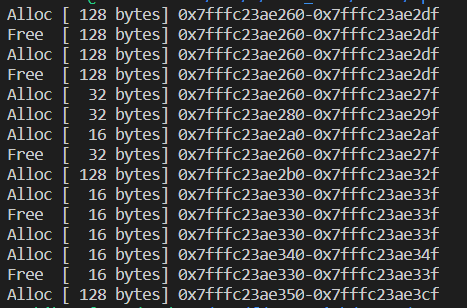
\includegraphics[scale = 0.7]{result.png}
\bigbreak

\par{This is how maps file look like:}
\\
\includegraphics[scale = 0.7]{maps.png}
\bigbreak

\par{The first column is the address corresponding to the last column which is the pathname, you can check if the output of the main.c source code is valid with the address given.}
\par{The second column is the perms field which is the set of the permission.}
\begin{itemize}
    \item r = read.
    \item w = write.
    \item x = execute.
    \item s = shared.
    \item p = private.
\end{itemize}

\par{The offset field is located in the third column}
\par{The next column is dev that is the device.}
\par{The next one is inode on that device 0 indicates that no inode is associated with the memory region.}

\section{References:}

\nocite{FAQ,gjaingjain,kerrisk_2012,pomerantz_2000,shared,tajiryan}
\bibliography{IEEEabrv, HelloWorld}
\bibliographystyle{IEEEtran}
%\printbibliography


\end{document}